\documentclass{article}

%% Page Margins %%
\usepackage{geometry}
\geometry{
    top = 0.75in,
    bottom = 0.75in,
    right = 0.75in,
    left = 0.75in,
}

\usepackage{amsmath}
\usepackage{graphicx}
\usepackage{parskip}

\title{Assembly Project: Dr Mario}

% TODO: Enter your name
\author{Maximilian Djaya}

\begin{document}
\maketitle

\section{Instruction and Summary}

\begin{enumerate}

    \item Which milestones were implemented?
    
    Milestones 1 and 2, with 3 partly done. Just not clearing rows and columns yet.
    \item How to view the game:
    % TODO: specify the pixes/unit, width and height of 
    %       your game, etc.  NOTE: list these details in
    %       the header of your breakout.asm file too!
    
    \begin{enumerate}

    \item Open DrMario.asm in MARS.
    \item Open the bitmap.
    \begin{enumerate}
        \item set the pixel height to 8
        \item set the pixel width to 8
        \item set the display width to 512
        \item set the display height to 512
        \item change the base address to 0x10008000
        \item click connect to MIPS.
    \end{enumerate}
    \item Open the keyboard input and click connect to MIPS.
    \item Assemble DrMario.asm and run.


    \end{enumerate}

    

\begin{figure}[ht!]
    \centering
    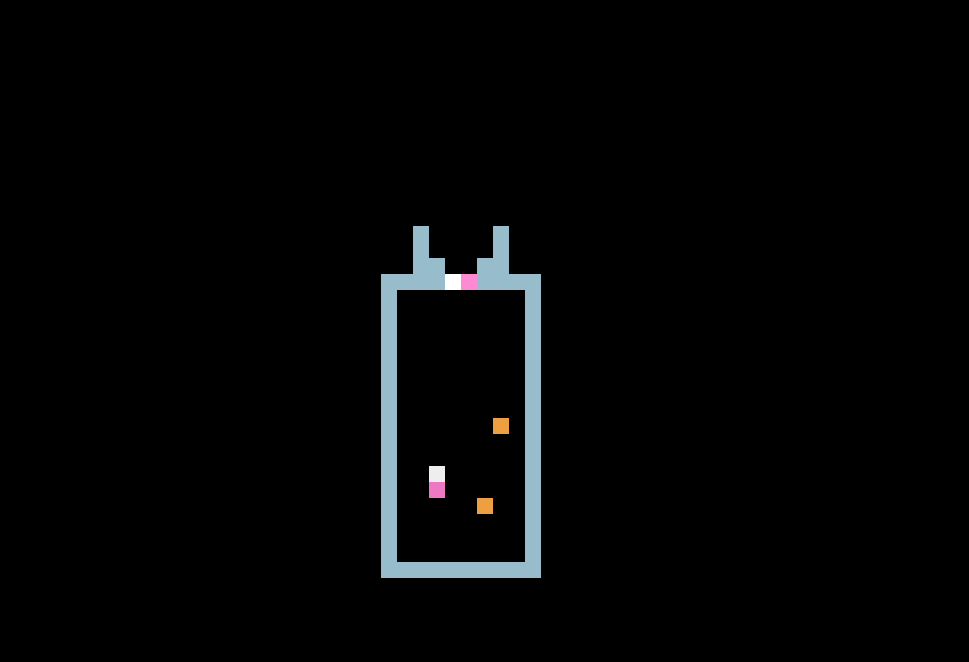
\includegraphics[width=0.3\textwidth]{initializedDrmario.png}
    \caption{What it should look like}
    \label{Instructions}
\end{figure}

\item Game Summary:
\begin{itemize}
\item It is just dr mario so far. (WASD to move)
\item I dont have it so that when there is a connection it clears yet
\end{itemize}

    
\end{enumerate}

\section{Attribution Table}
% TODO: If you worked in partners, tell us who was 
%       responsible for which features. Some reweighting 
%       might be possible in cases where one group member
%       deserves extra credit for the work they put in.

\begin{center}
\begin{tabular}{|| c ||}
\hline
 Maximilian Djaya (1010401744)\\ 
 \hline
 Everything
\end{tabular}
\end{center}

% TODO: Fill out the remainder of the document as you see 
%       fit, including as much detail as you think 
%       necessary to better understand your code. 
%       You can add extra sections and subsections to 
%       help us understand why you deserve marks for 
%       features that were more challenging than they
%       might initially seem.


\end{document}